%% -----------------------------------------------------------------------------

\chapter{Introduction}\label{ch:introduction}


%% -----------------------------------------------------------------------------

\section{Motivation}\label{sec:motivation}

In today's modern society, ...

Modern programming languages like Rust and Go have mechanisms to protect potential
unsafe usages, e.g., dereferences of raw pointers or modifying static variables. Thus, it is
recommended to avoid unsafe usages. However, if a developer wants to avoid unsafe
usages and potential security vulnerabilities caused by these usages, they do not only need
to check their code but also their dependencies.

To provide a developer the power to understand the unsafe usages within their code base,
tools like cargo-geiger~\cite{CargoGeiger} exists. Unfortunately, such a tool does not exist by today for Go.
Thus, an in-depth analysis of how many Go projects include direct and indirect unsafe
usages and if these projects are vulnerable does not exist, e.g., to buffer overflows~\cite{larochelle2001, alnaeli2017, wang2020}.
Within this work, the aim is to develop a tool, probably based on go vet~\cite{GoVet}, that can identify
unsafe usages in Go projects - similar to cargo-geiger. Based on this tool, the thesis should
evaluate how common unsafe usages in Go are and try to analyze if vulnerabilities caused
by unsafe usages exist.

\begin{figure}
    \centering
    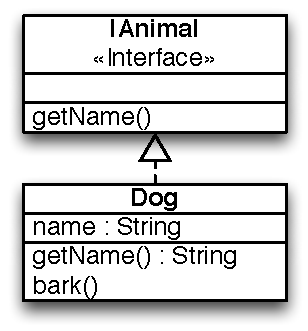
\includegraphics[width=4cm]{assets/images/uml}
    \caption{Sample UML Diagram}
    \label{fig:uml_example}
\end{figure}



%% -----------------------------------------------------------------------------

\section{Contributions}\label{sec:contributions}

The contributions of this thesis are:

\begin{enumerate}
    \item An analysis of unsafe code usage in the 500 most popular open-source Go projects,
    including the identification of (three) main areas of danger
    \item An in-depth analysis of consequences of those patterns with respect to a security
    context
    \item The submission of (14) fixes to previously vulnerable code snippets in open-source Go
    libraries, 10 of which have already been merged
    \item An open-source tool to identify unsafe usages in Go code including its dependencies
    \item An open-source, Go Vet-style, linter tool to find (two) unsafe usage patterns of \texttt{unsafe.Pointer}
    that were previously uncaught with existing tools
    \item (An IDE integration of these tools using plugins for JetBrains GoLand and Eclipse)
\end{enumerate}



%% -----------------------------------------------------------------------------

\section{Outline}\label{sec:outline}

This thesis is structured as follows: Chapter 2 gives background information on the motivation
and consequences of the safe and unsafe code language features, as well as its implementation
in the Go programming language.

Chapter 3 describes the dependency management system found in modern languages, specifically
the Go module system with respect to open source software.

Chapter 4 contains the design and implementation of a Go static analysis tool which can identify
unsafe code usages in the package as well as its dependencies.

Chapter 5 compares the analysis tool to related work on the Rust programming language and the
more general OWASP dependency checker.

Chapter 6 analyzes possible vulnerabilities caused by unsafe code usages, specifically with
respect to cryptographic APIs.

Chapter 7 contains a survey and analysis of the top 500 most popular open source Go projects
with respect to their usage of unsafe code in the project or its dependencies. It also has an
analysis of identified security vulnerabilities.

Finally, chapter 8 concludes the work with a discussion of the results and possible future work.